
\index{Optics|textbf}

This section describes advanced X-ray optics
components such as mirrors and analyzer crystals.
A description of the reflectivity of a mirror is found
in section~\ref{ss:mirrorreflect}.

\section{Mirror: The multilayer elliptic mirror}
\label{s:mirror}
\index{Optics!Mirror plane}
\component{Multilayer Elliptic Mirror}{System}{$\theta$, $s1$, $s2$, $length$, $width$, $R$}{}{validated}
%{$R_0, Q_c, W, \alpha, reflect$}{validated}

The component {\bf Multilayer Elliptic Mirror}
models a single rectangular reflecting multilayer mirror plate with elliptical curvature. It can be used
as a sample component, to \textit{e.g.}~assemble a Kirkpatrick-Baez focusing system 
or in combination with a double-crystal monochromator.


Figure~\ref{fig:Ellipse}\emph{Left} shows a side view of a mirror
(the blue section of the ellipse) in the McXtrace coordinate system.
At the mirror center, the mirror tangent is parallel to the $z$ axis
and the mirror normal is parallel to the $y$ axis. The width of the
mirror is $w$ and in $y-z$ plane the mirror has the curvature of an
ellipse with major axis $a$ and minor axis $b$,
%
\begin{equation} 
\frac{z^2}{ a^2} + \frac{y^2}{b^2} =1\,, \,|x| <
\frac{w}{2}\,.
\end{equation}
%
The length of the mirror is $L$. The coordinates of the mirror
center $(0,Y_0,Z_0)$ and the ellipse parameters $a$, $b$ are
determined uniquely by the central glancing angle, the source-mirror
distance and the mirror-image distance. The position of the mirror
is chosen to be at the positive side of the $y$ axis.

The input parameters of this component are:
$\theta$ [$^{\circ}$], the incident angle; 
$s1$ [m], the distance from the source to the multilayer;
$s2$ [m], the focusing distance of the multilayer;
$length$ [m], the length of the mirrors;
$width$ [m], the width of the mirror along the $x$-axis;
$R$, the reflectivity.

\subsection{Definition of the reference frames}
The direction and position of the incoming photon is defined
relative to the coordinate system illustrated in
Fig.~\ref{fig:Ellipse}\emph{Left} (in the code referred to as
\emph{McXtrace coordinate system}):
\begin{itemize}
\item the y-axis is parallel to the central mirror normal
\item the z-axis is parallel to the central mirror tangent
\item the origin is at the mirror center
\end{itemize}

However, all the calculations are conducted in another reference
frame which is illustrated in Fig.~\ref{fig:Ellipse}~\emph{Right}(in
the following referred to as the \emph{Ellipse coordinate system}):
\begin{itemize}
\item the z-axis is parallel to major axis of ellipse
\item the y-axis is parallel to minor axis of ellipse
\item the origin is at the center of the ellipse
\item the mirror center at $(0,Y_0,Z_0)$, uniquely determined by the
glancing angle at the mirror center, the source-mirror distance and
mirror-image distance.
\end{itemize}

\begin{figure}[htb!]
\centering
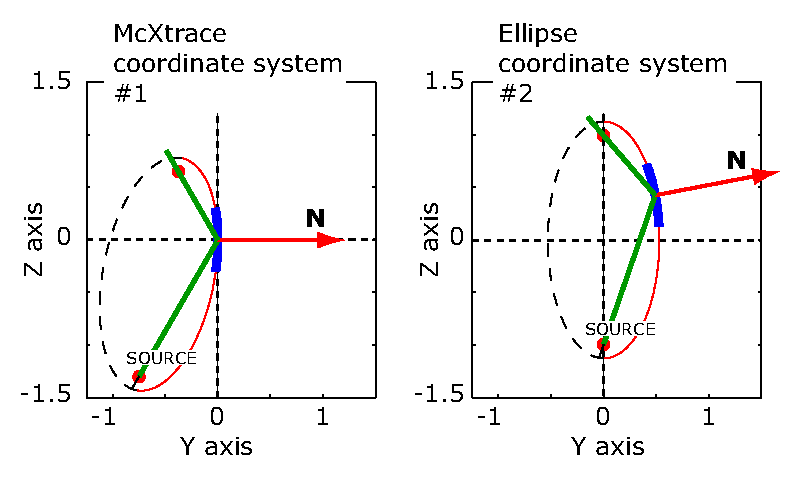
\includegraphics[width=0.95\linewidth]{figures/ellipse.eps}
 \caption{The same image in different coordinate systems.\newline \emph{Left}:
 \emph{McXtrace System} with the y-axis is parallel to the central mirror normal, the z-axis
 is parallel to the central mirror tangent and the origin is at the mirror
 center. \newline
 \emph{Right}: \emph{Ellipse System} with
the z-axis parallel to major axis of ellipse, the y-axis is parallel
to minor axis of ellipse and the origin is at the center of the
ellipse. }\label{fig:Ellipse}
\end{figure}


\subsection{Algorithm}
\begin{enumerate}
\item The photon is generated with a starting point $\bf{S}$ and a direction
$\bf{V}_\textrm{in}$ defined in the \emph{McXtrace} coordinate
system.
\item All calculations are performed in the \emph{Ellipse} coordinate system,
so to proceed the basis is changed to that reference frame.
\item The 2 intersections of the ray with the ellipse are determined.
\item It is checked if any of the intersections are within the area
defined by the mirror.
\item If one of the solutions is valid, the reflection of that ray is
determined.
\item The coordinates of the starting point and direction of the
reflected ray are calculated using the basis of the \emph{McXtrace}
coordinate system.
\end{enumerate}


\section{Reflection of the ray in the mirror}
\begin{figure}[htb!]
\centering
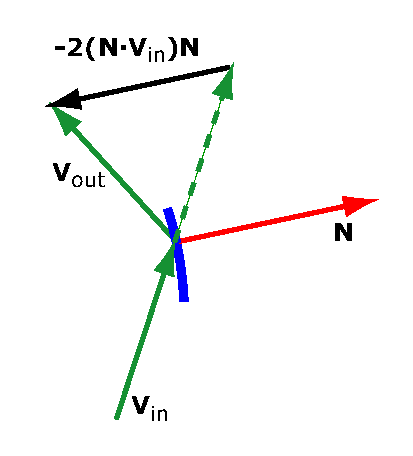
\includegraphics[width=0.3\linewidth]{figures/Dotproduct.eps}
 \caption{The reflection of the unit vector $\bf{V}_\textrm{in}$ in the mirror with the normal unit
 vector ${\bf{N}}$ is ${\bf{V}}_\textrm{out} = {\bf{V}}_\textrm{in} -2({\bf{N}}\cdot{\bf{V}}_\textrm{in}){\bf{N}}$}\label{fig:dotProduct}
\end{figure}

The tangent and normal to the ellipse $z^2/a^2 + y^2/b^2=1$ at the
point $(Y,Z)$ are found by implicit differentiation: \begin{equation} 
\frac{2z}{a^2} + \frac{2y}{b^2} \,\frac{dy}{dz} = 0\,, \end{equation} so at the
point $(Y,Z)$ the slope of the tangent is $\frac{dy}{dz} =
-\frac{Z\,b^2}{Y\,a^2}$. The slope of the normal is minus the
inverse of the tangent slope, so the coordinates of the mirror
normal are \begin{equation} N_x = 0 \quad N_y = \frac{a^2\,Y}{b^2\,Z} \quad N_z =
1\,. \end{equation} With $\bf{V}_\textrm{in}$ and $\bf{N}$ denoting unit
vectors (direction and normal respectively), the direction of the
reflected ray is calculated as \begin{equation} {\bf{V}}_\textrm{out} =
{\bf{V}}_\textrm{in} -2({\bf{N}}\cdot{\bf{V}}_\textrm{in}){\bf{N}} =
        \left(
      \begin{array}{c}
        V_{\textrm{in}x} - 2({\bf{N}}\cdot{\bf{V}}_\textrm{in})N_x \\
               V_{\textrm{in}y} - 2({\bf{N}}\cdot{\bf{V}}_\textrm{in})N_y \\
                V_{\textrm{in}z} - 2({\bf{N}}\cdot{\bf{V}}_\textrm{in})N_z \\
      \end{array}
    \right)
\end{equation}


\subsection{Mirror reflectivity}
\label{ss:mirrorreflecttable}


At present, the Multilayer Elliptic Mirror component uses a reflectivity table $reflect$, 
which 1st column is q [$\AA^{-1}$] and from the 2nd column on as the reflectivity $R$ in [0-1]
as function of tabulated energy [$KeV$]. 
An example file, calculated for a particular $Si/W$ multilayer, is provided (\verb+reflectivity.txt+).
User provided reflectivity data files can be parsed by the component.

\subsection{Mirror reflectivity calculation}
\label{ss:mirrorreflect}


To compute the reflectivity of the neutron supermirrors instead, we use an empirical
formula derived from experimental data \cite{pb_241_50},
see Fig.~\ref{f:reflectivity}. The reflectivity is given by
\begin{equation} \label{e:Rmirror}
  R = \left\{
    \begin{array}{ll}
      R_0 & \textrm{if $Q \leq Q_{\rm c}$} \\
      \frac{1}{2}R_0(1 - \tanh[(Q - m Q_{\rm c})/W])(1-\alpha(Q-Q_{\rm c}))
         & \textrm{if $Q > Q_{\rm c}$}
    \end{array}
  \right.
\end{equation}

Here $Q$ is the length of the scattering vector (in \AA$^{-1}$)
defined by
\begin{equation} \label{e:reflectivity}
Q = |{\bf k}_{\bf i} - {\bf k}_{\bf f}|
  = \frac{m_{\rm n}}{\hbar} |{\bf v}_{\bf i} - {\bf v}_{\bf f}|,
\end{equation}
$m_{\rm n}$ being the neutron mass.
The number $m$ in (\ref{e:Rmirror}) is a parameter determined by
the mirror materials,
the bilayer sequence, and the number of bilayers.
As can be seen, $R=R_0$ for $Q < Q_{\rm c}$, where $Q_{\rm c}$ is the
critical scattering wave vector for a single layer of the mirror
material. At higher values of $Q$, the reflectivity starts falling
linearly with a slope $\alpha$ until a "soft cut-off" at $Q = m Q_{\rm c}$.
The width of this cut-off is denoted $W$. See the example reflection curve in
figure~\ref{f:reflectivity}.

It is {\bf important} to notice that when $m < 1$, the reflectivity remains constant at $R=R_0$ up to $q=Qc$, and \emph{not} $m.Q_c$. This means that $m < 1$ parameters behave like $m=1$ materials.

Alternatively, the Mirror, Guide and Guide\_gravity components may use a reflectivity table $reflect$, which 1st column is q [$\AA^{-1}$] and 2nd column as the reflectivity $R$ in [0-1]. For this purpose, we provide $m=2$ and $m=3$ reflectivity files from SwissNeutronics (\verb+supermirror_m2.rfl+ and \verb+supermirror_m3.rfl+ in \verb+MCSTAS/lib/data/+).

\subsection{Algorithm}
The function of the component can be described as
\begin{enumerate}
\item Propagate the neutron ray to the plane of the mirror.
\item If the neutron trajectory intersects the mirror plate, it is
reflected, otherwise it is left untouched.
\item Reflection of the incident velocity
${\bf v}_{\rm i} = (v_x,v_y,v_z)$
gives the final velocity ${\bf v}_{\rm f} = (v_x,v_y,-v_z)$.
\item Calculate $Q=2 m_{\rm n} v_z / \hbar$.
\item The neutron weight is adjusted with the amount $\pi_i = R(Q)$.
\item  To avoid spending large amounts of computation time on very low-weight
neutrons, neutrons for which the reflectivity is lower than about
$10^{-10}$ are ABSORB'ed.
\end{enumerate}

\begin{figure}
  \begin{center}
    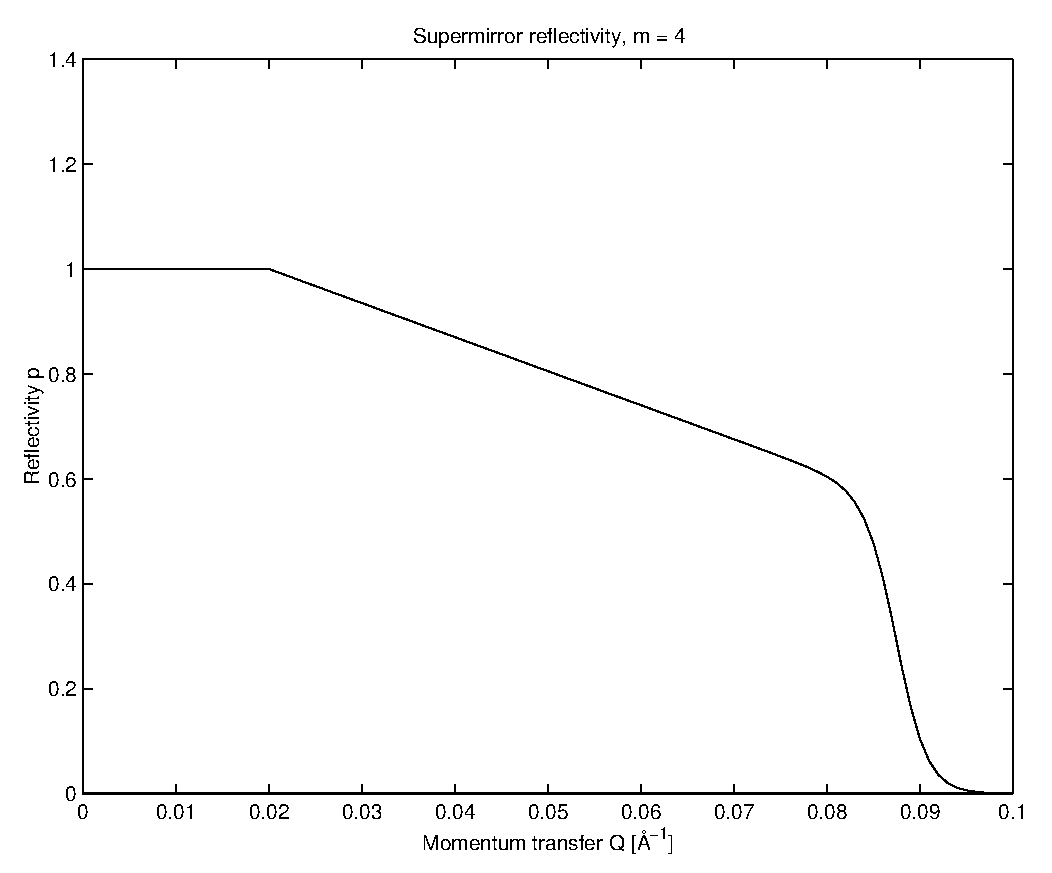
\includegraphics[width=0.6\textwidth]{figures/supermirror.eps}
  \end{center}
\caption{A typical reflectivity curve for a supermirror,
Eq.~(\protect\ref{e:reflectivity}). The used values are
$ m=4$, $R_0=1$, $Q_{\rm c} = 0.02$~\AA$^{-1}$, $\alpha = 6.49$~\AA,
$ W=1/300$~\AA$^{-1}$.
}
\label{f:reflectivity}
\end{figure}

\newpage

\section{Guide: The guide section}
\index{Optics!Straight guide}

\component{Guide}{System}{$w_1, h_1$, $w_2, h_2$, $l$, $m$, $reflect$}{$R_0, Q_c, W, \alpha$}{validated, no gravitation support}

The component {\bf Guide}
models a guide tube consisting of four flat mirrors. The
guide is centered on the $z$ axis with rectangular entrance and exit
openings parallel to the $x$-$y$ plane. The entrance has the dimensions
$(w_1,h_1)$ and placed at $z=0$. The exit is of dimensions $(w_2,h_2)$
and is placed at $z=l$ where $l$ is the guide length. See
figure~\ref{f:guide}.
The reflecting properties are given by the values of
$R_0, m, Q_c, W$, and $\alpha$, as for {\bf Mirror}, or alternatively from the reflectivity file $reflect$.

{\bf Guide} may produce wrong results with gravitation support.
Use {\bf Guide\_gravity} (section \ref{s:guide_gravity}) in this case,
or the {\bf Guide\_channeled}
in section~\ref{s:channeled_guide}.

\begin{figure}
  \begin{center}
    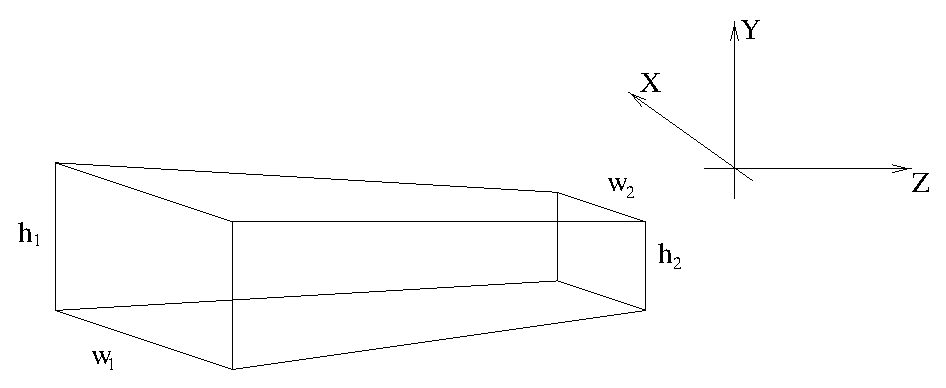
\includegraphics[width=0.7\textwidth]{figures/guide1.eps}
  \end{center}
\caption{The geometry used for the guide component.}
\label{f:guide}
\end{figure}

\subsection{Guide geometry and reflection}
For computations on the guide geometry, we define the planes of the four
guide sides by giving their normal vectors (pointing into the guide)
and a point lying in the plane:
$$
\begin{array}{rclcrcl}
{\bf n}^v_1 &=& (l, 0, {(w_2 - w_1) / 2})
     & & {\bf O}^v_1 &=& (- w_1 / 2, 0, 0) \\
{\bf n}^v_2 &=& (-l, 0, {(w_2 - w_1) / 2})
     & & {\bf O}^v_2 &=& (w_1 / 2, 0, 0) \\
{\bf n}^h_1 &=& (0, l, {(h_2 - h_1) / 2})
     & & {\bf O}^h_1 &=& (0, - h_1 / 2, 0) \\
{\bf n}^h_2 &=& (0, -l, {(h_2 - h_1) / 2})
     & & {\bf O}^h_2 &=& (0, h_1 / 2, 0) \\
\end{array}
$$
In the following, we refer to an arbitrary guide side by its origin
{\bf O} and normal {\bf n}.

With these definitions, the time of intersection of the neutron with a
guide side can be computed by considering the projection onto the
normal:
\begin{equation}
t^\alpha_\beta = \frac{({\bf O}^\alpha_\beta - {\bf r}_0) \cdot {\bf n}^\alpha_\beta}
  {{\bf v} \cdot {\bf n}^\alpha_\beta}  ,
\end{equation}
where $\alpha$ and $\beta$ are indices for the different guide walls,
assuming the values (h,v) and (1,2), respectively.
For a neutron that leaves the guide directly through the guide exit we have
\begin{equation}
t_{\rm exit} = \frac{l - z_0}{v_z}
\end{equation}

The reflected velocity ${\bf v}_{\rm f}$ of the neutron with incoming velocity
${\bf v}_{\rm i}$ is computed by the formula
\begin{equation}
 {\bf v}_{\rm f} =
  {\bf v}_{\rm i}
   - 2{{\bf n} \cdot \frac{{\bf v}_{\rm i}}{{|{\bf n}|^2}} {\bf n}}
\end{equation}
This expression is arrived at by again considering the projection onto
the mirror normal (see figure~\ref{f:guidereflect}). The reflectivity of the
mirror is taken into account as explained in section~\ref{s:mirror}.

\begin{figure}
  \begin{center}
    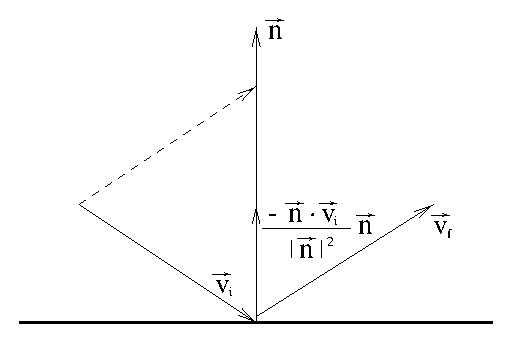
\includegraphics[width=0.5\textwidth]{figures/guide2.eps}
  \end{center}
\caption{Neutron reflecting from mirror. ${\bf v}_{\rm i}$ and
${\bf v}_{\rm f}$ are the initial and final velocities, respectively,
and {\bf n} is a vector normal to the mirror surface.}
\label{f:guidereflect}
\end{figure}

\subsection{Algorithm}
\begin{enumerate}
\item The neutron is initially propagated to the $z = 0$ plane of the
guide entrance.
\item If it misses the entrance, it is ABSORB'ed.
\item Otherwise, repeatedly compute the time of intersection with the
four mirror sides and the guide exit.
\item The smallest positive $t$ thus
found gives the time of the next intersection with the guide (or in the
case of the guide exit, the time when the neutron leaves the guide).
\item Propagated the neutron ray to this point.
\item Compute the reflection from the side.
\item Update the neutron weight factor by the amount $\pi_i = R(Q)$.
\item Repeat this process until the neutron leaves the guide.
\end{enumerate}

There are a few optimizations possible here to avoid redundant
computations. Since the neutron is always inside the guide during the
computations, we always have
$({\bf O} - {\bf r}_0) \cdot {\bf n} \leq 0$.
Thus $t \leq 0$ if ${\bf v} \cdot {\bf n} \geq 0$, so in this case
there is no need to actually compute $t$. Some redundant computations
are also avoided by utilizing symmetry and the fact that many
components of {\bf n} and {\bf O} are zero.

\newpage

\section{Guide\_channeled: A guide section component with multiple channels}
\label{s:channeled_guide}
\index{Optics!Guide with channels (straight, non focusing)}

\component{Guide\_channeled}{System}{$w_1, h_1$, $w_2, h_2$, $l$, $k$, $m_x, m_y$}{$d, R_0, Q_{cx}, Q_{cy}, W, \alpha_x, \alpha_y$}{validated, no gravitation support}

The component {\bf Guide\_channeled} is a more complex variation of {\bf Guide}
described in the previous section. It allows the specification
of different supermirror parameters for the horizontal and vertical
mirrors, and also implements guides with multiple channels as used in
neutron bender devices. By setting the $m$ value of the supermirror
coatings to zero, nonreflecting walls are simulated;
this may be used for a very detailed simulation of a Soller collimator,
see section~\ref{collimator-linear}.

The input parameters are $w_1$, $h_1$, $w_2$, $h_2$, and $l$
to set the guide dimensions as for {\bf Guide}
(entry window, exit window, and length);
$k$ to set the number of channels; $d$ to set the thickness of the
channel walls; and $R_0$, $W$, $Q_{cx}$, $Q_{cy}$, $\alpha_x$, $\alpha_y$,
$m_x$, and $m_y$ to set the supermirror parameters as described under {\bf Guide}
(the names with \textit{x} denote the vertical mirrors,
and those with \textit{y} denote the horizontal ones).

\subsection{Algorithm}
The implementation is based on that of {\bf Guide}.
\begin{enumerate}
\item Calculate the channel which the neutron will enter.
\item Shift the $x$ coordinate so that the channel can be simulated
as a single instance of the {\bf Guide} component.
\item (do the same as in {\bf Guide}.)
\item Restore the coordinates when the
neutron exits the guide or is absorbed.
\end{enumerate}

\subsection{Known problems}\index{Bugs}
\begin{itemize}
\item This component may produce wrong results with gravitation support.
Use Guide\_gravity (section \ref{s:guide_gravity}) in this case.
\item The focusing channeled geometry (for $k > 1$ and different
values of $w_1$ and $w_2$) is buggy
(wall slopes are not computed correctly, and the component 'leaks' neutrons).
\end{itemize}
\newpage

\section{Guide\_gravity: A guide with multiple channels and gravitation handling}
\label{s:guide_gravity}
\index{Optics!Guide with channels and gravitation handling (straight)}
\index{Optics!Fermi Chopper}

\component{Guide\_gravity}{System}{$w_1, h_1$, $w_2, h_2$, $l$, $k$, $m$}{$d, R_0, Q_c, W, \alpha$, wavy, chamfers, $k_h$, $n$, $G$}{validated, {\bf with} gravitation support, rotating mode}

This component is a variation of {\bf Guide\_channeled}
(section \ref{s:channeled_guide}) with the ability to handle
gravitation effects and functional channeled focusing geometry.
Channels can be specified in two dimensions,
producing a 2D array ($k, k_h$) of smaller rectangular guide channels.

The coating is specified as for the Guide and Mirror components by mean of the parameters $R_0, m, Q_c, W$, and $\alpha$, or alternatively from the reflectivity file $reflect$.

Waviness effects, supposed to be randomly distributed
(\emph{i.e.} non-periodic waviness)
can be specified globally, or for each part of the guide section.
Additionally, chamfers
may be defined the same way.
Chamfers originate from the substrate manufacturing, so that operators do not harm themselves with cutting edges. Usual dimensions are about tens of millimeters. They are treated as absorbing edges around guide plates, both on the input and output surfaces, but also aside each mirror.

The straight section of length $l$ may be divided into $n$ bits of same length
within which chamfers are taken into account.

The component has also the capability to rotate at a given frequenccy in order to approximate a Fermi Chopper, including phase shift. The approximation resides in the fact that the component is considered fixed during neutron propagation inside slits. Beware that this component is then located at its entry window (not centered as the other Fermi choppers).\index{Bugs}

To activate gravitation support, either select the \MCS\ gravitation support (\verb+mcrun --gravitation ...+ or from the Run dialog of \verb+mcgui+),
or set the gravitation field strength $G$ (e.g. -9.81 on Earth).

This component is about 50 \% slower than the \verb+Guide+ component, but has much more capabilities.

A contributed version Guide\_honeycomb of this component exists with a honeycomb geometry.

\section{Bender: a bender model (non polarizing)}
\index{Optics!Bender (non polarizing)}

\component{Bender}{Philipp Bernhardt}{$r, W_{in},l,w,h $}{$k,d,R_{0[a,i,s]},\alpha_{[a,i,s]},m_{[a,i,s]},Q_{c[a,i,s]},W_{[a,i,s]}$}{partly validated, no gravitation support}

The Bender component is simulating an ideal curved neutron guide (bender). It is bent to the negative X-axis and behaves like a parallel guide in the Y axis. Opposite curvature may be achieved by a $(0,0,180)$ rotation (along Z-axis).

Bender radius $r$, entrance width $w$ and height $h$ are required parameters. To define the length, you may either enter the deviation angle $W_{in}$ or the length $l$. Three different reflectivity profiles $R_0,Q_c,W,m,\alpha$ can be given (see section~\ref{s:mirror}): for outer
walls (index $a$), for inner walls (index $i$) and for the top and bottom walls (index $s$).

To get a better transmission coefficient, it is possible to split the bender into $k$ channels which are separated by partitions with the thickness of $d$. The partitioning walls have the same coating as the exterior walls.

Because the angle of reflection doesn't change, the routine
calculates the reflection coefficent for the concave and, if necessary, for the convex wall only onces, together with the number of reflections.
Nevertheless the exact position, the time, and the divergence is calculated at the end of the bender, so there aren't any approximations.

The component is shown \emph{straight} on geometrical views (mcdisplay/Trace), and the next component may be placed directly at distance $r.W_{in} = l$ \emph{without} rotation.

Results have been compared succesfully with analytical formula in the case of an ideal reflection and cross-checked with the program \verb+haupt+.

An other implementation of the Bender is available as the contributed component Guide\_curved.

\section{Curved guides}
\index{Optics!Curved guides (polygonal model)}

Real curved guides are usually made of many straight elements (about 1 m long) separated with small gaps (e.g. 1 mm). Sections of about 10 m long are separated with bigger gaps for accessibility and pumping purposes.

We give here an example description of such a section. Let us have a curved guide of total length $L$, made of $n$ elements with a curvature radius $R$. Gaps of size $d$ separate elements from each other. The rotation angle of individual straight guide elements is $\alpha_z = (L+d)/R*180/\pi$ in degrees.

In order to build an independent curved guide section, we define \verb+Arm+ components at the begining and end of it.
\begin{verbatim}
COMPONENT CG_In = Arm() AT (...)

COMPONENT CG_1  = Guide_gravity(l=L/n, ...)
AT (0,0,0) RELATIVE PREVIOUS

COMPONENT CG_2  = Guide_gravity(l=L/n, ...)
AT (0,0,L/n+d) RELATIVE PREVIOUS
ROTATED (0, (L/n+d)/R*180/PI, 0) RELATIVE PREVIOUS
...
COMPONENT CG_Out = Arm() AT (0,0,L/n) RELATIVE PREVIOUS
\end{verbatim}
The \verb+Guide+ component should be duplicated $n$ times by copy-paste, but changing the instance name, e.g. CG\_1, CG\_2, ..., CG\_n. This may be automated with the \verb+COPY+ or the \verb+JUMP ITERATE+ mechanisms (see User manual).

An implementation of a continuous curved guide has been contributed as component Guide\_curved.

